% main.tex
\documentclass{Report} % 使用您自定义的类

% --- 设置所有封面和页眉的占位符信息 ---
\ReportLogo{ZJU.jpg} % 您的代码指定了 ZJU.jpg
\Major{信息工程}
\StudentName{何~铭~源}
\StudentID{3240104481}
\ReportDate{\today}
\ReportLocation{紫金港东四219}

\CourseName{电子电路设计实验I}
\TeacherName{施红军、叶险峰、邓靖靖}
\ExperimentName{叠加定理实验研究} % 此项也会用于页眉
\ExperimentType{验证类实验}
\TeamMate{孙潇枫}
\newcolumntype{C}{>{\centering\arraybackslash}c}
\begin{document}


\makecover

\section{实验目的}
\begin{enumerate}
    \item 定量研究验证叠加定理的正确性。并加深对电路理论的理解。

    \item 掌握直流电路的基本连接、电压和电流的测量方法。
\end{enumerate}

\section{实验任务和要求}
\begin{enumerate}
    \item 使用理论计算出电路中各个支路的电流值与各个节点的电压值
    \item 使用电流表，电压表测量实际值，并与理论值进行对比，验证叠加原理的正确性
\end{enumerate}
\section{实验原理}
\begin{itemize}
    \item \textbf{适用范围：} 仅适用于\textbf{线性电路}。

    \item \textbf{核心思想：}
    在线性电路中，任一支路的电流（或任两点间的电压），等于各个独立电源\textbf{单独作用}时，在该处产生的电流（或电压）的\textbf{代数和}。

    \item \textbf{“单独作用”处理方式：}
    \begin{itemize}
        \item \textbf{理想电压源：} 置零，即\textbf{短路}。
        \item \textbf{理想电流源：} 置零，即\textbf{开路}。
        \item \textbf{受控源：} 始终保留。
    \end{itemize}

    \item \textbf{重要限制：}
    \begin{itemize}
        \item \textbf{非线性网络：} 定理\textbf{不成立}。
        \item \textbf{功率计算：} \textbf{不能}直接用于计算功率。
        \item \textbf{原因：} 功率是二次量（如 $P = I^2R$ 或 $P = V^2/R$），不满足线性叠加。
    \end{itemize}

\end{itemize}
\section{实验方案设计与参数计算}
\subsection{实验方案总体设计}
\begin{figure}[H]
\centering
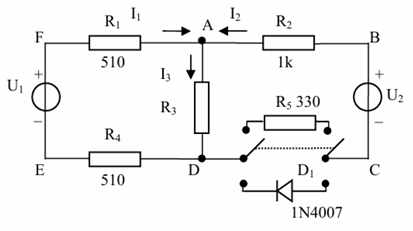
\includegraphics[width=0.6\textwidth]{./fig/基尔霍夫.png}
\caption{设计电路验证叠加定理}
\label{fig}
\end{figure}
本次实验的核心目的是利用\cref{fig}所示的电路，来对叠加定理进行实验验证，并探究其适用范围。
在开始测量之前，我们首先需要明确电路分析的参考方向，特别是图1中标明的三个主要支路电流（$I_1, I_2, I_3$）的方向。
在后续测量中保持此参考方向不变，是进行电流代数和比较的基础。
实验中，我们采用了两路直流稳压电源 $U_{s1}$ 和 $U_{s2}$，并将它们的输出电压均设定为 6V。
实验内容分为两部分：首先，将电阻 $R_5$（线性元件）接入电路。我们将分别测量两个电源（$U_{s1}, U_{s2}$）共同作用时的电流，以及它们各自单独作用（另一电源置零/短路）时的电流。通过比较“共同作用”的测量值是否等于两个“单独作用”测量值的代数和，来验证叠加定理的成立。
接着，我们将 $R_5$ 替换为二极管 $D_1$（非线性元件），并完整地重复上述所有测量步骤。
通过比较数据，我们将观察并证明叠加定理在非线性电路中将不再适用。
\subsection{理论值计算}
\subsubsection{接入$R$}
\paragraph{当 $U_1$ 和 $U_2$ 共同作用时}
\begin{equation}
\begin{cases}
    1020I_1 + 510I_3 = 6 \\
    1330I_2 + 510I_3 = 12 \\
    I_1 + I_2 = I_3
\end{cases}
\end{equation}

解得

\begin{equation}
\begin{cases}
    I_1 = 1.92\,\text{mA} \\
    I_2 = 5.988\,\text{mA} \\
    I_3 = 7.914\,\text{mA}
\end{cases}
\end{equation}

由电流的结果可以依次算出 $U_1 = 6\text{V}, U_2 = 12\text{V}, U_{FA} = 0.982\text{V}, U_{AB} = -5.988\text{V}, U_{AD} = 4.036\text{V}, U_{CD} = -1.995\text{V}, U_{DE} = 0.982\text{V}$。

\paragraph{仅 $U_1$ 单独作用时 ($U_2$ 短路)}
\begin{equation}
\begin{cases}
    1020I_1 + 510I_3 = 6 \\
    I_2 = 0 \\
    I_1 = I_3
\end{cases}
\end{equation}

解得

\begin{equation}
\begin{cases}
    I_1 = 3.922\,\text{mA} \\
    I_2 = 0 \\
    I_3 = 3.922\,\text{mA}
\end{cases}
\end{equation}

由电流的结果可以依次算出 $U_1 = 6\text{V}, U_2 = 0\text{V}, U_{FA} = 2\text{V}, U_{AB} = 0, U_{AD} = 2\text{V}, U_{CD} = 2\text{V}, U_{DE} = 2\text{V}$。
\paragraph{仅 $U_2$ 单独作用时 ($U_1$ 短路)}
\begin{equation}
\begin{cases}
    1020I_1 + 510I_3 = 6 \\
    1330I_2 + 510I_3 = 0 \\
    I_1 + I_2 = I_3
\end{cases}
\end{equation}

\begin{equation}
\begin{cases}
    I_1 = 4.32\,\text{mA} \\
    I_2 = -1.20\,\text{mA} \\
    I_3 = 3.12\,\text{mA}
\end{cases}
\end{equation}

由电流结果可以依次算出 $U_1 = 6\text{V}, U_2 = 0\text{V}, U_{FA} = 2.20\text{V}, U_{AB} = 1.20\text{V}, U_{AD} = 1.59\text{V}, U_{CD} = 0.39\text{V}, U_{DE} = 2.21\text{V}$。

\subsubsection{接入$D$}
\paragraph{当 $U_1$ 和 $U_2$ 共同作用时}
\begin{equation}
\begin{cases}
    1020I_1 + 510I_3 = 0 \\
    1330I_2 + 510I_3 = 12 \\
    I_1 + I_2 = I_3
\end{cases}
\end{equation}

\begin{equation}
\begin{cases}
    I_1 = -2.40\,\text{mA} \\
    I_2 = 7.19\,\text{mA} \\
    I_3 = 4.79\,\text{mA}
\end{cases}
\end{equation}

从而依次可以推出 $U_1 = 0\text{V}, U_2 = 12\text{V}, U_{FA} = -1.224\text{V}, U_{AB} = -7.19\text{V}, U_{AD} = 2.443\text{V}, U_{CD} = -2.367\text{V}, U_{DE} = -1.219\text{V}$。
\paragraph{仅 $U_1$ 单独作用时 ($U_2$ 短路)}
\begin{equation}
\begin{cases}
    1020I_1 + 510I_3 = 6 \\
    I_2 = 0 \\
    I_1 = I_3
\end{cases}
\end{equation}

解得

\begin{equation}
\begin{cases}
    I_1 = 3.922\,\text{mA} \\
    I_2 = 0 \\
    I_3 = 3.922\,\text{mA}
\end{cases}
\end{equation}

由电流的结果可以依次算出 $U_1 = 6\text{V}, U_2 = 12\text{V}, U_{FA} = 2\text{V}, U_{AB} = 0, U_{AD} = 2\text{V}, U_{CD} = -10\text{V}, U_{DE} = 2\text{V}$。
\paragraph{仅 $U_2$ 单独作用时 ($U_1$ 短路)}
\begin{equation}
\begin{cases}
    1020I_1 + 510I_3 = 0 \\
    I_2 = 0 \\
    I_1 = I_3
\end{cases}
\end{equation}

解得：
\[I_1 = I_2 = I_3 = 0\]

由此可以算出 $U_1 = 0\text{V}, U_2 = 12\text{V}, U_{FA} = 0\text{V}, U_{AB} = 0, U_{AD} = 0\text{V}, U_{CD} = -12\text{V}, U_{DE} = 0\text{V}$

\section{实验仪器设备}
\begin{itemize}
    \item 万用表
    \item 电流表
    \item 实验室提供的电路板
\end{itemize}
\section{实验步骤、实验数据记录}
\subsection{当 $R_5$ 接入时}

% ---------------------------------------------------
% 表 1: U1 单独作用
% ---------------------------------------------------
\begin{table}[H]
\centering
\caption{$U_1$ 单独作用}
\label{tab:U1_alone}
\resizebox{\textwidth}{!}{% 缩放表格以适应页面宽度
\begin{tabular}{l *{10}{C}}
\toprule
 & $U_1$ & $U_2$ & $I_1$ & $I_2$ & $I_3$ & $U_{FA}$ & $U_{AB}$ & $U_{AD}$ & $U_{CD}$ & $U_{DE}$ \\
\midrule
理论值 & $6\text{V}$ & $0$ & $4.32\text{mA}$ & $-1.20\text{mA}$ & $3.12\text{mA}$ & $2.20\text{V}$ & $1.20\text{V}$ & $1.59\text{V}$ & $0.39\text{V}$ & $2.21\text{V}$ \\
测量值 & $6.00\text{V}$ & $0$ & $4.36\text{mA}$ & $1.18\text{mA}$ & $3.16\text{mA}$ & $2.16\text{V}$ & $1.18\text{V}$ & $1.58\text{V}$ & $0.39\text{V}$ & $2.24\text{V}$ \\
\bottomrule
\end{tabular}
}
\end{table}

% ---------------------------------------------------
% 表 2: U2 单独作用
% ---------------------------------------------------
\begin{table}[H]
\centering
\caption{$U_2$ 单独作用}
\label{tab:U2_alone}
\resizebox{\textwidth}{!}{% 缩放表格以适应页面宽度
\begin{tabular}{l *{10}{C}}
\toprule
 & $U_1$ & $U_2$ & $I_1$ & $I_2$ & $I_3$ & $U_{FA}$ & $U_{AB}$ & $U_{AD}$ & $U_{CD}$ & $U_{DE}$ \\
\midrule
理论值 & $0$ & $12\text{V}$ & $-2.40\text{mA}$ & $7.19\text{mA}$ & $4.79\text{mA}$ & $-1.224\text{V}$ & $-7.19\text{V}$ & $2.443\text{V}$ & $-2.367\text{V}$ & $-1.219\text{V}$ \\
测量值 & $0$ & $12.00\text{V}$ & $2.36\text{mA}$ & $7.17\text{mA}$ & $4.78\text{mA}$ & $-1.17\text{V}$ & $-7.18\text{V}$ & $2.39\text{V}$ & $-2.42\text{V}$ & $-1.22\text{V}$ \\
\bottomrule
\end{tabular}
}
\end{table}

% ---------------------------------------------------
% 表 3: U1, U2 共同作用
% ---------------------------------------------------
\begin{table}[H]
\centering
\caption{$U_1, U_2$ 共同作用}
\label{tab:U1_U2_together}
\resizebox{\textwidth}{!}{% 缩放表格以适应页面宽度
\begin{tabular}{l *{10}{C}}
\toprule
 & $U_1$ & $U_2$ & $I_1$ & $I_2$ & $I_3$ & $U_{FA}$ & $U_{AB}$ & $U_{AD}$ & $U_{CD}$ & $U_{DE}$ \\
\midrule
理论值 & $6\text{V}$ & $12\text{V}$ & $1.926\text{mA}$ & $5.988\text{mA}$ & $7.914\text{mA}$ & $0.982\text{V}$ & $-5.988\text{V}$ & $4.036\text{V}$ & $-1.995\text{V}$ & $0.982\text{V}$ \\
测量值 & $6.00\text{V}$ & $12.01\text{V}$ & $2.00\text{mA}$ & $5.99\text{mA}$ & $7.95\text{mA}$ & $0.99\text{V}$ & $-6.00\text{V}$ & $3.98\text{V}$ & $-2.03\text{V}$ & $1.03\text{V}$ \\
\bottomrule
\end{tabular}
}
\end{table}

% ---------------------------------------------------
% 表 4: 汇总表 (根据新的测量值)
% ---------------------------------------------------
\begin{table}[H]
\centering
\caption{汇总表}
\label{tab:summary_measured}
\resizebox{\textwidth}{!}{% 缩放表格以适应页面宽度
\begin{tabular}{l *{10}{C}}
\toprule
 & $U_1$ & $U_2$ & $I_1$ & $I_2$ & $I_3$ & $U_{FA}$ & $U_{AB}$ & $U_{AD}$ & $U_{CD}$ & $U_{DE}$ \\
\midrule
$U_1$ 单独作用 & $6.00\text{V}$ & $0$ & $4.36\text{mA}$ & $1.18\text{mA}$ & $3.16\text{mA}$ & $2.16\text{V}$ & $1.18\text{V}$ & $1.58\text{V}$ & $0.39\text{V}$ & $2.24\text{V}$ \\
$U_2$ 单独作用 & $0$ & $12.00\text{V}$ & $2.36\text{mA}$ & $7.17\text{mA}$ & $4.78\text{mA}$ & $-1.17\text{V}$ & $-7.18\text{V}$ & $2.39\text{V}$ & $-2.42\text{V}$ & $-1.22\text{V}$ \\
$U_1$ 和 $U_2$ 共同作用 & $6.00\text{V}$ & $12.01\text{V}$ & $2.00\text{mA}$ & $5.99\text{mA}$ & $7.95\text{mA}$ & $0.99\text{V}$ & $-6.00\text{V}$ & $3.98\text{V}$ & $-2.03\text{V}$ & $1.03\text{V}$ \\
\bottomrule
\end{tabular}
}
\end{table}

\section*{接入 $D_1$，重复上述测量：}

% ---------------------------------------------------
% 表 5: U1 单独作用 (D1)
% ---------------------------------------------------
\begin{table}[H]
\centering
\caption{$U_1$ 单独作用}
\label{tab:U1_alone_D1}
\resizebox{\textwidth}{!}{% 缩放表格以适应页面宽度
\begin{tabular}{l *{10}{C}}
\toprule
 & $U_1$ & $U_2$ & $I_1$ & $I_2$ & $I_3$ & $U_{FA}$ & $U_{AB}$ & $U_{AD}$ & $U_{CD}$ & $U_{DE}$ \\
\midrule
理论值 & $6\text{V}$ & $0$ & $3.922\text{mA}$ & $0$ & $3.922\text{mA}$ & $2\text{V}$ & $0$ & $2\text{V}$ & $2\text{V}$ & $2\text{V}$ \\
测量值 & $6.00\text{V}$ & $0$ & $4.31\text{mA}$ & $-0.97\text{mA}$ & $3.25\text{mA}$ & $2.14\text{V}$ & $1.04\text{V}$ & $1.63\text{V}$ & $0.58\text{V}$ & $2.22\text{V}$ \\
\bottomrule
\end{tabular}
}
\end{table}

% ---------------------------------------------------
% 表 6: U2 单独作用 (D1)
% ---------------------------------------------------
\begin{table}[H]
\centering
\caption{$U_2$ 单独作用}
\label{tab:U2_alone_D1}
\resizebox{\textwidth}{!}{% 缩放表格以适应页面宽度
\begin{tabular}{l *{10}{C}}
\toprule
 & $U_1$ & $U_2$ & $I_1$ & $I_2$ & $I_3$ & $U_{FA}$ & $U_{AB}$ & $U_{AD}$ & $U_{CD}$ & $U_{DE}$ \\
\midrule
理论值 & $0$ & $12\text{V}$ & $0$ & $0$ & $0$ & $0$ & $0$ & $0$ & $-12\text{V}$ & $0$ \\
测量值 & $0$ & $12.01\text{V}$ & $0$ & $0$ & $0$ & $0$ & $0$ & $0$ & $-12.01\text{V}$ & $0$ \\
\bottomrule
\end{tabular}
}
\end{table}

% ---------------------------------------------------
% 表 7: U1, U2 共同作用 (D1)
% ---------------------------------------------------

\begin{table}[H]
\centering
\caption{$U_1, U_2$ 共同作用}
\label{tab:U1_U2_together_D1}
\resizebox{\textwidth}{!}{% 缩放表格以适应页面宽度
\begin{tabular}{l *{10}{C}}
\toprule
 & $U_1$ & $U_2$ & $I_1$ & $I_2$ & $I_3$ & $U_{FA}$ & $U_{AB}$ & $U_{AD}$ & $U_{CD}$ & $U_{DE}$ \\
\midrule
理论值 & $6\text{V}$ & $12\text{V}$ & $3.922\text{mA}$ & $0$ & $3.922\text{mA}$ & $2\text{V}$ & $0$ & $2\text{V}$ & $-10\text{V}$ & $2\text{V}$ \\
测量值 & $6.00\text{V}$ & $12.01\text{V}$ & $3.96\text{mA}$ & $0\text{mA}$ & $3.96\text{mA}$ & $1.97\text{V}$ & $0$ & $1.98\text{V}$ & $-10.03\text{V}$ & $2.04\text{V}$ \\
\bottomrule
\end{tabular}
}
\end{table}

% ---------------------------------------------------
% 表 8: 汇总表 (D1, 根据新的测量值)
% ---------------------------------------------------

\begin{table}[H]
\centering
\caption{汇总表}
\label{tab:summary_measured_D1}
\resizebox{\textwidth}{!}{% 缩放表格以适应页面宽度
\begin{tabular}{l *{10}{C}}
\toprule
 & $U_1$ & $U_2$ & $I_1$ & $I_2$ & $I_3$ & $U_{FA}$ & $U_{AB}$ & $U_{AD}$ & $U_{CD}$ & $U_{DE}$ \\
\midrule
$U_1$ 单独作用 & $6.00\text{V}$ & $0$ & $4.31\text{mA}$ & $-0.97\text{mA}$ & $3.25\text{mA}$ & $2.14\text{V}$ & $1.04\text{V}$ & $1.63\text{V}$ & $0.58\text{V}$ & $2.22\text{V}$ \\
$U_2$ 单独作用 & $0$ & $12.01\text{V}$ & $0$ & $0$ & $0$ & $0$ & $0$ & $0$ & $-12.01\text{V}$ & $0$ \\
$U_1$ 和 $U_2$ 共同作用 & $6.00\text{V}$ & $12.01\text{V}$ & $3.96\text{mA}$ & $0\text{mA}$ & $3.96\text{mA}$ & $1.97\text{V}$ & $0$ & $1.98\text{V}$ & $-10.03\text{V}$ & $2.04\text{V}$ \\
\bottomrule
\end{tabular}
}
\end{table}



\section{数据分析与讨论}
\begin{itemize}
    \item 对于接入电阻，有汇总的表格中前两行数据之和大致等于第三行，也就是说叠加定理成立。但对于非线性元件，第三行不等于前两行之和，对于非线性电路，叠加定理失效。
    \item 本次实验的总体误差不大。
    \item 接入二极管后，当 $U_1$ 单独供电时，测得 $I_2 > 0$。此现象或因二极管存在漏电流，或源于测量仪器本身的误差。
    \item 实验过程中，电压源的输出存在起伏，这也为测量带来了误差。
\end{itemize}

\section{结论}
实验证明，只有在线性电路中，电路中的电压与电流遵循叠加定理。

叠加定理对于非线性电路不适用，实验数据也验证了这一点。而且，功率并不满足叠加定理。

\section{心得与体会}
本次实验涉及的测量考量点多，计算过程相对繁琐，且测量次数频繁。
我深刻体会到了耐心与细心的重要性，
同时，我的实验操作与测量技能也得到了锻炼。

\section{思考题}

\subsection{是否能通过直接短路的方式将未工作的电源（U1 或 U2）置零？}

不可行。因为短接电源会导致其内部流过极大电流，进而损坏电源。

\subsection{依据实验数据，计算在不同条件下，某一电阻所消耗的功率，并检验功率是否满足叠加性。}

以 $R_1$ ($R_1 = 510 \Omega$) 为例，计算其消耗的功率：
\begin{itemize}
    \item $U_1$ 单独作用时：$P_1 = I_1^2 \times R_1 = ((4.36 \times 10^{-3})^2 \times 510 = 9.695 \times 10^{-3} \text{ W}$
    \item $U_2$ 单独作用时：$P_2 = I_2^2 \times R_1 = ((-2.36 \times 10^{-3})^2 \times 510 = 2.840 \times 10^{-3} \text{ W}$
    \item $U_1$ 与 $U_2$ 共同作用时：$P_{12} = I_3^2 \times R_1 = ((2.00 \times 10^{-3})^2 \times 510 = 2.040 \times 10^{-3} \text{ W}$
\end{itemize}

显然 $P_1 + P_2 = 9.695 \times 10^{-3} \text{ W} + 2.840 \times 10^{-3} \text{ W} = 12.535 \times 10^{-3} \text{ W} \neq P_{12}$。
故推出功率不具有叠加性。
\end{document}